% !TeX root = text.tex
\chapter{hardware}
Tato kapitola se zabývá fyzickou konstrukcí a zapojením vyrobeného laserového projektoru. Ten se skládá z řídící jednotky, galvanometrů s~ovládací elektronikou, laseru, chlazení a napájení. Všechny tyto součástky jsou uloženy v pouzdře vytisknutém na 3D tiskárně.

\section{Řídící jednotka -- Raspberry Pi}
\fxnote{TODO: rpi specs}

\section{Set galvanometrů se~zrcátky} \label{sec:my-galvos}
\subsection{Výběr skeneru}
Pro tuto práci byl vybrán galvanometrový skener, protože je~nejdostupnější a~protože potenciálním uživatelům nejlépe představí technologii.

Oproti hranolovým skenerům jim tožiž dává více možností, jak s paprskem pohybovat.
Můžou se~rozhodnout, že jej využijí jako hranolový skener, pokud nahrají soubor procházející promítací plochu po~řádcích.

Oproti dalším typům skenerů je~názornější, ostatní typy skenerů jsou totiž příliš malé a~není na~nich vidět princip funkce nebo je~jejich fungování nadmíru abstraktní a~těžko pochopitelné.

\subsection{Zapojení galvanometrového setu}
Samotné galvanometry jsou zapojeny do~řídící desky, která s nimi byla zakoupena, ta je vidět na obrázku~\ref{fig:hw_galvoboard}.

Řídící deska požaduje symetrický zdroj napětí 15~V, tzn. $+15$~V a~$-15$~V a~samozřejmě připojení k zemi. Také přijímá dva bipolární diferenciální analogové signály s~rozsahem diferenciálního napětí $-10$~V až $+10$~V. Každý signál udává vychýlení jednoho ze~dvou galvanometrů, což obvykle znamená výslednou pozici laserového paprsku v~osách X~a~Y.

\begin{figure}[htb]
  \centering
  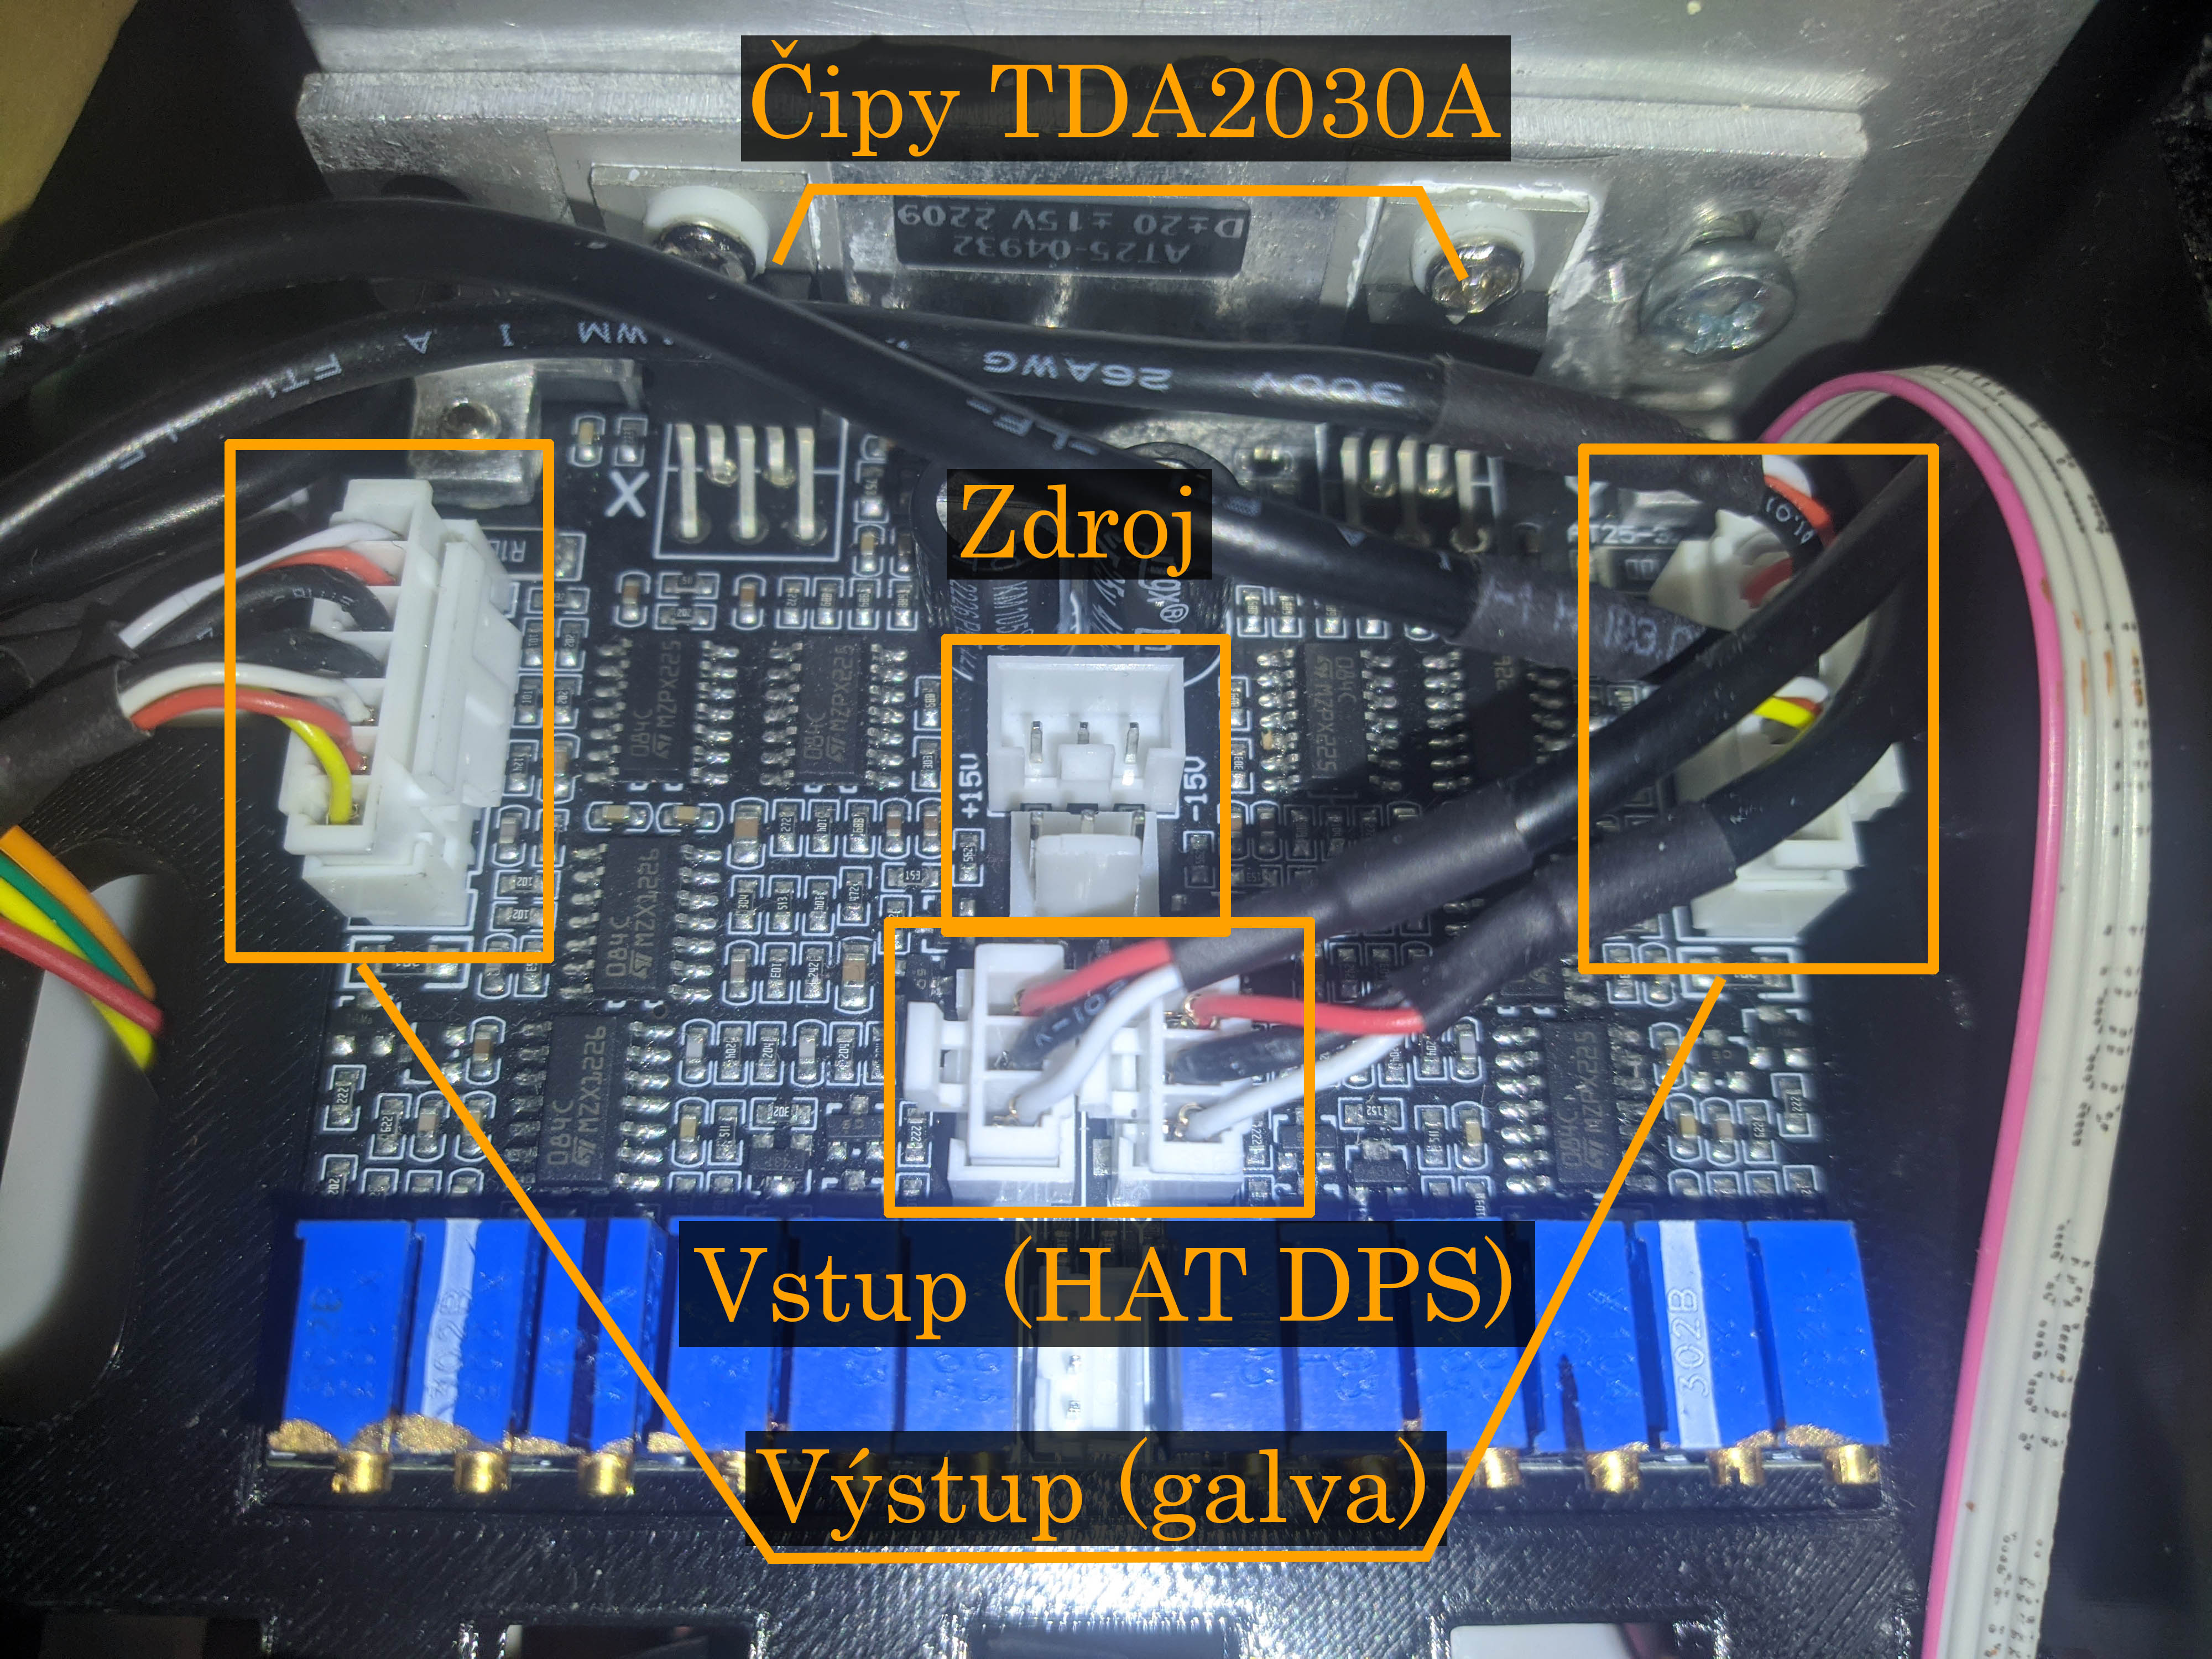
\includegraphics[width=1\textwidth]{img/hw_galvoboard.jpg}
  \caption{\label{fig:hw_galvoboard} Řídící deska galvanometrů s vyznačenými konektory a hřejícími čipy}
\end{figure}

\subsection{Bipolární diferenciální analogový signál}
Diferenciální signál je~signál přenášený dvěma vodiči, každý z~nich přenáší stejný signál, jen s~opačnou polaritou. Kontakt označený $(+)$ je~považován za~nosič základního signálu, zatímco kontakt označený $(-)$ je~považován za~nosič invertovaného signálu. Výsledné diferenciální napětí je~napětí na~základním nosiči vůči napětí na~obráceném nosiči, tzn.~$V_{dif} = V_{(+)} - V_{(-)}$.~\cite{ilda-signal-spec}

Bipolární signál znamená, že na~napětí každém z~kontaktů $(+)$ a~$(-)$ může dosahovat kladných i~záporných hodnot~\cite{ilda-signal-spec}.

Tudíž cheme-li disáhnout diferenciálního napětí $+10~V$, musí mít základní signál napětí $+5~V$ a~obrácený signál $-5~V$. Záporné diferenciální napětí bude ve~chvíli, kdy je~napětí základního signálu záporné a~napětí obráceného signálu kladné.

\subsection{Zahřívání čipů řídící desky galvanometrů} \label{sec:galvoboard-chips-heating-up}
Dva z~čipů na~řídící desce se při chodu systému výrazně zahřívájí. Na~tyto čipy je naštěstí už od~výroby desky připevněna malá hliníková destička. Ta~má sloužit jako chladič, ale i~s ní se~čipy v~otevřeném prostoru zahřívají na~teploty blízké 60~\degree{}C.
Dva zmíněné čipy jsou čipy TDA2030A od~firmy STMicroelectronics. Ty~by~měly dle datasheetu vydržet až 150~\degree{}C, ale dá se~předpokládat, že v~uzavřeném pouzdru budou čipy dosahovat vyšších teplot, než v~otevřeném prostoru. I~kdyby nedosáhly pro sebe kritických 150~\degree{}C, rozhodně není žádoucí, aby uvnitř projektoru desky dosahovaly vysokých teplot.

I proto byl do~projektoru zabudován chladič. Více o~způsobu jeho připevnění a~distribuci chlazení mezi ostatní komponenty se~dočtete v~kapitole~\ref{sec:krabick-design-priorities}.


\section{laser}
Jako zdroj laserového paprsku byl využit RGB laserový modul, skládající se ze tří barevných diod a dichroických zrcátek.

\subsection{Dichroická zrcadla~\cite{dichronic-mirrors}}

\fxnote{TODO: slouzi k}

Dichroická zrcadla jsou zrcadla s výrazně rodílnými odrazovými nebo průchodovými vlastnostmi pro dvě různé vlnové délky odraženého~/~procházejícího světla.

Většina dichroických zrcadel jsou dielektrická zrcádla \footnote{Dielektrická zrcadla jsou zrcadla, skládající se z mnoha tenkých vrstev různě opticky propustných materiálů.}, existují ale také krystalická zrcadla\footnote{Krystalická zrcadla jsou zrcadla, jejiž odrážlivá vrstva se skládá z monokrystalického materiálu, typicky polovodiče.}.


\section{Displej z~tekutých krystalů (LCD)}
Pro zobrazování informací uživateli přímo na~zařízení byl~využit alfanumerický\footnote{Alfanumerický -- Řídící jednotka displeji místo pixelů posílá celé znaky, které sám vykresluje.} LCD~s řadičem HD44780 a~s~rozlišením 20~x~4 znaky. K~displeji je~také připojen I$^{2}$C převodník, který slouží jako prostředník mezi řadičem displeje a~Raspberry Pi.
Komunikační protokol LCD~totiž využívá podstatně více kontaktů, než I$^{2}$C sběrnice, kterou Raspberry Pi~komunikuje s~převodníkem.
% Převodník je~k~pinům Raspberry Pi~připojen dle~tabulky~\ref{tab:LCD_conn}.

\begin{figure}[htb]
  \centering
  \begin{minipage}{0.45\textwidth}
    \centering
    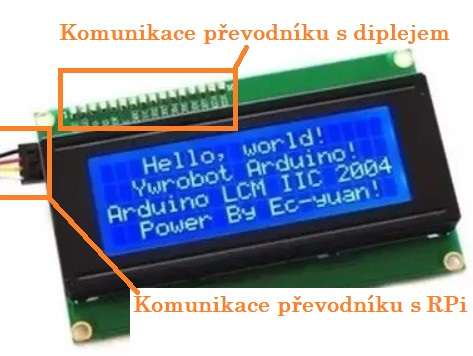
\includegraphics[width=1\textwidth]{img/LCD_front.jpg} % first figure itself
    \caption{\label{fig:LCD_front} Displej z~tekutých krystalů (LCD); Převzato a~upraveno z~\cite{laskakit-LCD}}
  \end{minipage}\hfill
  \begin{minipage}{0.45\textwidth}
    \centering
    \includegraphics[width=1\textwidth]{img/LCD_back.jpg} % second figure itself
    \caption{\label{fig:LCD_back} I$^{2}$C převodník napojený na~LCD~\cite{laskakit-LCD}}
  \end{minipage}
\end{figure}

% \begin{table}[htb]
%   \centering
%   \begin{tabular}{c|c}
%     kontakt převodníku & kontakt RPi~\\
%     \hline
%      GND~               & GND~        \\
%     5V                 & 5V          \\
%      SCK~               & GPIO3       \\
%      SDA~               & GPIO2       \\
%      LED~               & GPIO18      \\
%   \end{tabular}
%   \caption{\label{tab:LCD_conn} Připojení kontaktů I$^{2}$C převodníku na~kontakty RPi.}
% \end{table}


\section{Rotační enkodér}
Rotační enkodér je~typ~pozičního senzoru používaný k~měření rotace otáčivé hřídele~\cite{how-encoders-work}. Existuje mnoho druhů enkodérů, rozdělují se~dle~signálu, který vydávají a~dle~technologie, kterou měří rotaci hřídele~\cite{how-encoders-work}. V~této práci je~použit mechanický inkrementální enkodér s~tlačítkem.

Na obrázku~\ref{fig:encoder-working} je~vidět, jak~enkodér funguje uvnitř. Dva~kontakty A~a~B při rotaci získávají a~ztrácí kontakt s~kontaktem C. Připojíme-li ke~kontaktu C~zem a~ke~kontaktům A~a~B pull-up rezistory (klidně softwarově), dá se~toto získávání a~ztrácení kontaktu zaznamenat do~grafu na~obrázku~\ref{fig:encoder-graph} jako dva~signály obdélníkového průběhu vzájemně fázově posunuté o~90 stupňů.

\begin{figure}[htb]
  \centering
  \begin{minipage}{0.45\textwidth}
    \centering
    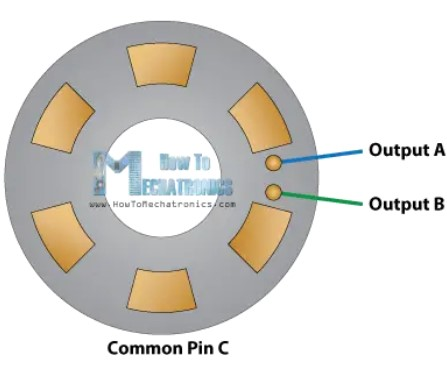
\includegraphics[width=1\textwidth]{img/encoder-working.jpg}
    \caption{\label{fig:encoder-working} Vnitřní schéma enkodéru~\cite{how-encoders-work}}
  \end{minipage}\hfill
  \begin{minipage}{0.45\textwidth}
    \centering
    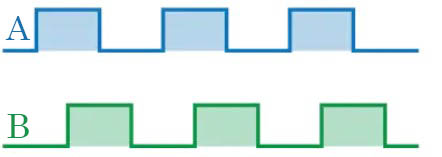
\includegraphics[width=1\textwidth]{img/encoder-graph.jpg}
    \caption{\label{fig:encoder-graph} Výstup enkodéru~\cite{how-encoders-work}}
  \end{minipage}
\end{figure}

Použitý rotační enkodér má další dva~kontakty připojené k~tlačítku pod~rotující hřídelí.
Ke~čtení stisknutí tlačítka je~potřeba připojit jeden kontakt k~zemi, tedy ke~kontaktu C~a~druhý kontakt na~pull-up rezistor (klidně softwarově).
Celé zapojení enkodéru je~naznačeno na~obrázku~\ref{fig:encoder-pinout}. Kontakty tlačítka jsou v~něm označeny S1 a~S2.
% Enkodér je~k~RPi připojen dle~tabulky~\ref{tab:enc_conn}.

% \begin{table}[htb]
%   \centering
%   \begin{tabular}{c | c}
%     kontakt enkodéru & kontakt RPi~\\
%     \hline
%      C~               & GND~        \\
%     S2               & GND~        \\
%     A~               & GPIO5       \\
%      SDA~             & GPIO6       \\
%     S1               & GPIO13      \\
%   \end{tabular}
%   \caption{\label{tab:enc_conn} Připojení kontaktů rotačního enkodéru na~kontakty RPi.}
% \end{table}


\subsection{Čtení pozice z~rotačního enkodéru}
U rotačního enkodéru se~při každé otáčce změní připojení pinů několikkrát. Chceme-li pozorovat pouze počet těchto změn, stačí spočítat změny na~jednom kontaktu. Pokud je~ale~zapotřebí pozorovat i~směr otáčení, je~nutné pozorovat stav obou kontaktů. Pokud se~enkodér otáčí po~směru hodinových ručiček, kontakt A~bude fázově posunut o~90 stupňů napřed oproti kontaktu B.
Pokud se~eknodér otáčí proti směru hodinových ručiček, bude naopak kontakt B~o 90 stupňů napřed oproti kontaktu A. Časový průběh stavu kontaktů je~naznačen na~obrázku~\ref{fig:encoder_data}.
\begin{figure}[htb]
  \centering
  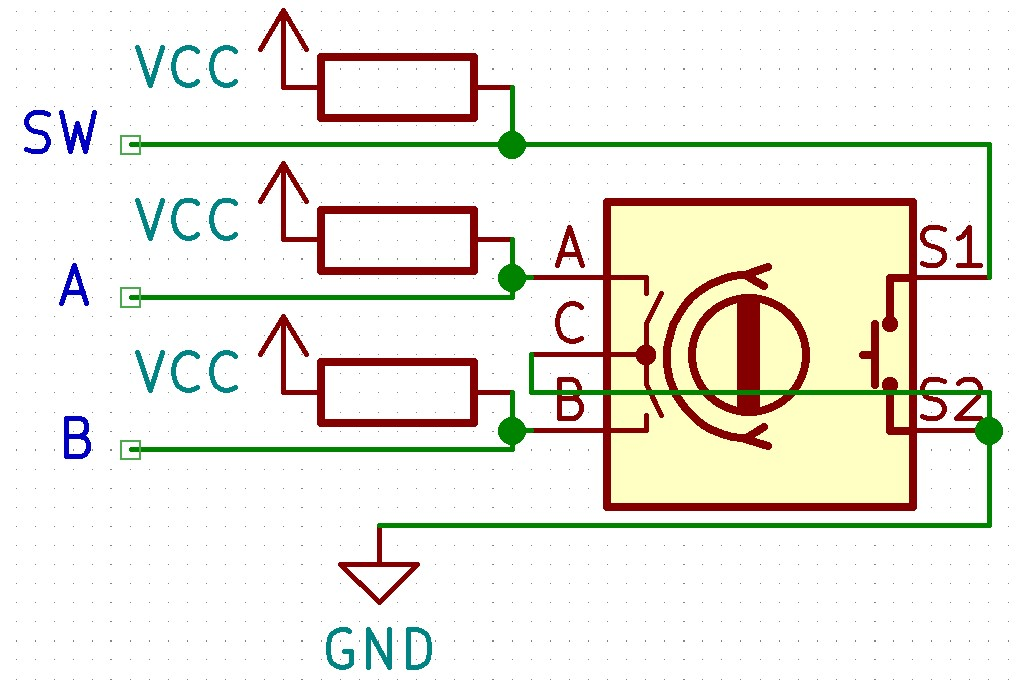
\includegraphics[width=0.5\textwidth]{img/encoder-pinout.jpg}
  \caption{\label{fig:encoder-pinout} Schéma zapojení rotačního enkodéru.}
\end{figure}
\begin{figure}[htb]
  \centering
  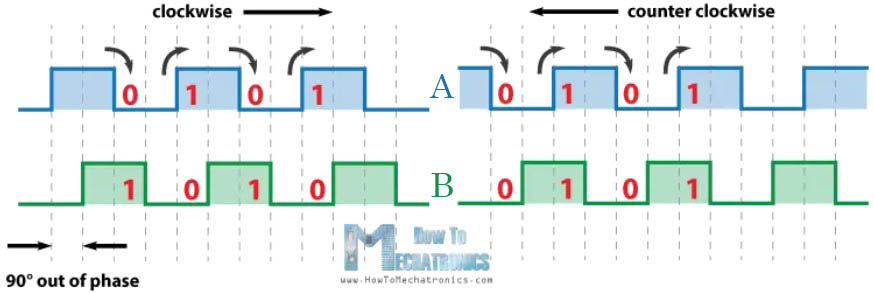
\includegraphics[width=1\textwidth]{img/encoder_data.jpg}
  \centering
  \caption{\label{fig:encoder_data} Časový průběh stavu kontaktů rotačního enkodéru při otáčení hřídelí na~obě strany}
\end{figure}


\section{HAT deska plošných spojů}
Pro ovládání výše popsaného hardwaru je~zapotřebí několik specifických obvodů.
Kvůli jejich specifičnosti tyto obvody nejsou volně dostupné k~zakoupení na~předem vytvořených destičkách. Proto bylo zapotřebí je~z~jednotlivých součástek vyrobit na~míru.

Obvody byly navrženy v~programu KiCad, celé schéma desky je k nalezení mezi přílohami s označením~\ref{fig:pcb-schematic-full}. Následně pro ně v~tomtéž programu byla nadesignována deska plošných spojů. Mezi obvody patří:
\begin{itemize}
  \item Zdroj $-15$~V pro galvanometry.
  \item Generátor signálu pro řídící desku galvanometrů.
  \item Voltmetr baterií.
\end{itemize}

Kromě nich byly na~desku přidány konektory k~jednotlivým barevným vstupům laseru, LCD displeji a~k rotačnímu enkodéru, které jsou přímo napojeny na~40 pinový GPIO konektor Raspberry Pi.
Deska byla designována jako tzv. HAT, to~znamená, že sama na~tomto konektoru drží a~nezabírá o~moc víc místa, než samotné Raspberry Pi.
\fxnote{TODO: obrazek desky (maybe mounted) (deska ještě nedošla)}

\subsection{Zdroj $-15$~V}\label{sec:negative-ps}
Napětí $-15$~V je získáváno obvodem napěťového invertoru založeném na obvodu ze zdroje~\cite{ampalyzer}. Jeho zapojení je na obrázku~\ref{fig:negative-ps}, potřebuje zdroj napětí 15V.

\begin{figure}[htb]
  \centering
  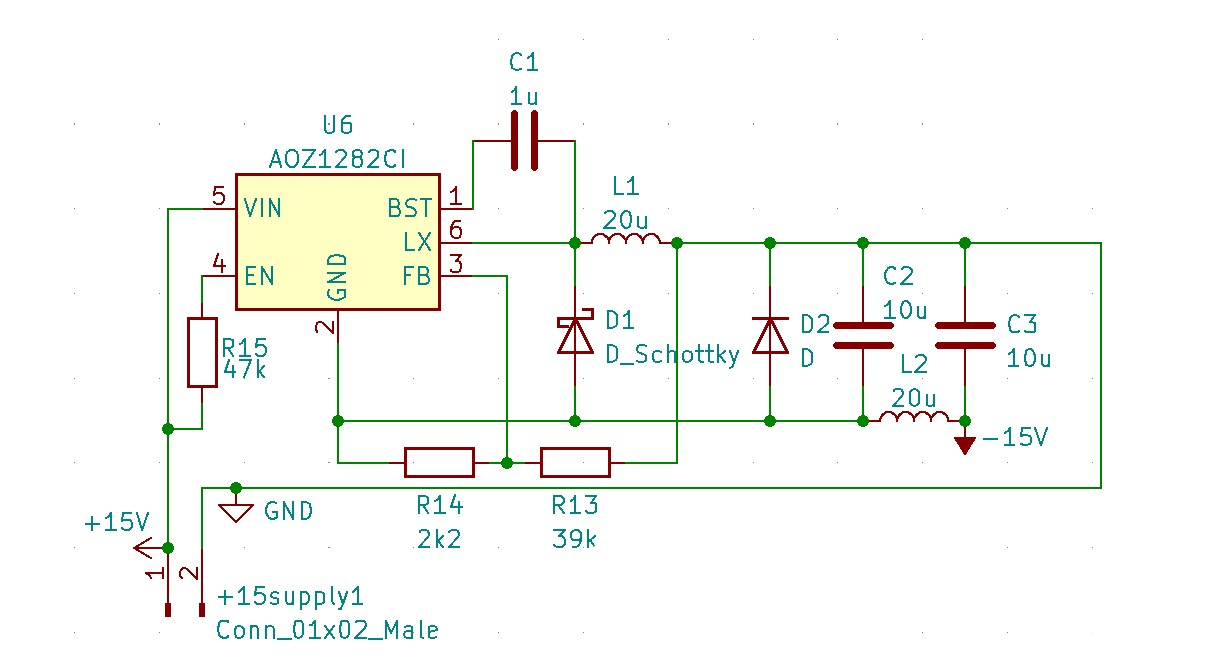
\includegraphics[width=0.9\textwidth]{img/negative-ps.jpg}
  \caption{\label{fig:negative-ps} Zapojení invertujícího obvodu}
\end{figure}

Centrem obvodu je integrovaný obvod AOZ1282 od výrobce Alpha \& Omega Semiconductor označený U6. Tento integrovaný obvod obsahuje spínací transistor (ve zjednodušeném schématu prvek SW), PWM regulační obvod pracující na frekvenci 450 kHz s napěťovou referencí 0,8 V, který reguluje čas připojení induktoru L1.
K němu je připojen bootstrapový kondenzátor C1, ten zajišťuje plovoucí buzení pro integrovaný spínač.
Dále je k němu připojený výkonový induktor L1, jehož hodnota byla zvolena dle rovnic uvedených ve zdroji~\cite{basic-calc-boost}, respektive podle dále uvedené rovnice~\ref{equ:inductor-calc}.~\cite{ampalyzer}

\begin{equ}[H]
  \centering
  \begin{math}
    L = \frac{-U_{OUT}\times U_{IN}}{0,4 \times 2 \times I_{OUT} \times f_{s} \times \left ( U_{IN} - U_{OUT} \right )} = \frac{- \left (-15 V \right )\times 15 V}{0,4 \times 2 \times 1 A \times 450 kHz \times \left ( 15 V - \left (-15 V \right ) \right )} \approx 21 \mu H
  \end{math}
  \caption{\label{equ:inductor-calc} Výpočet ideální indukčnosti cívky pro invertující obvod}
\end{equ}

\It{
  L --- Indukčnost spínaného induktoru \\
  U$_{IN}$ --- Vstupní napětí do invertujícího obvodu \\
  U$_{OUT}$ --- Výstupní napětí z invertujícího obvodu \\
  I$_{OUT}$ --- Výstupní proud z invertujícího obvodu \\
  f$_{s}$ --- Frekvence spínacího regulátoru \\
}

Na FB pin integrovaného obvodu je připojen napěťový dělič tvořený odpory R13 a R14, který integrovanému obvodu dodává zpětnou vazbu o výstupním napětí.
Hodnoty R13 a R14 jsou voleny tak, aby při 15 V, tedy požadovaném výstupním napětí, bylo na výstupu děliče napětí 0,8 V, tedy referenční napětí integrovaného spínaného regulátoru.
Schottkyho dioda SS56, označená D1, slouží k zadržení změny polarity induktoru. Usměrňovací dioda D2 je v propustném stavu při prvotním spuštění měniče, kdy je přes ní napájen U1 po dobu náběhu výstupního záporného napětí.
Posledním prvkem je výstupní vyhlazovací filtr tvořený kondenzátory C3 a C4 společně s induktorem L2.
Jeho úkol je minimalizovat výstupní napěťového zvlnění zdroje.~\cite{ampalyzer}

\subsection{Generátor analogového signálu}\label{sec:ilda-signal-gen}
Jak je popsáno v~sekci~\ref{sec:my-galvos}, řídící deska galvanometrů přijmá dva bipolární diferenciální analogové signály v~rozpětí $-5$~V až $+5$~V.

Obvod, který se~stará o~vytváření tohoto signálu, je~založený na~obvodu ze~zdroje~\cite{lasershow-with-real-galvos}.
Vytváření tohoto signálu je~rozděleno do~dvou částí. Nejdříve D/A~převodník připojený k~RPi vytvoří signál v~rozpětí 0 až 5~V a~následně je~tento signál pomocí invertujících operačních zesilovačů převeden na~požadované rozpětí a invertován.
Jednotlivé části tohoto obvodu jsou blíže popsány v~následujících kapitolách.

\subsubsection{D/A převodník}
K generování signálu v~rozpětí 0--5~V byl využit dvoukanálový D/A převodník\footnote{D/A převodník je obvod, který na~základě instrukcí přijatých digitálně generuje analogové napětí.} MCP4822.
Tento čip podporuje komunikaci přes rozhraní SPI, pracuje s~napájecím napětím 5~V a~s 12bitovým rozlišením (je schopen vygenerovat 4~096 různých napětí) na~dvou kanálech~\cite{mcp4822-dsh}.
RPi komunikuje s~čipem pomocí rozhraní SPI popsaném v kapitole~\ref{sec:spi}.

\subsubsection{Operační zesilovače~\cite{tl082-dsh}}
K modifikaci signálu z~DAC na~bipolární diferenciální analogový signál slouží pro každý kanál jeden čip TL082, který obsahuje dva operační zesilovače. Ty~jsou zapojeny dle schématu na~obrázku~\ref{fig:ilda_amps-scheme}.

Signál první operační zesilovač zesílí/zeslabí a~vertikálně posune dle nastavení potenciometrů Ygain (zesílení) a~Yoffset (posun) a~zároveň invertuje. Tento invertovaný signál následně druhý operační zesilovač opět invertuje. Tím získavá základní signál pro řídící desku galvanometrů.

\begin{figure}[htb]
  \centering
  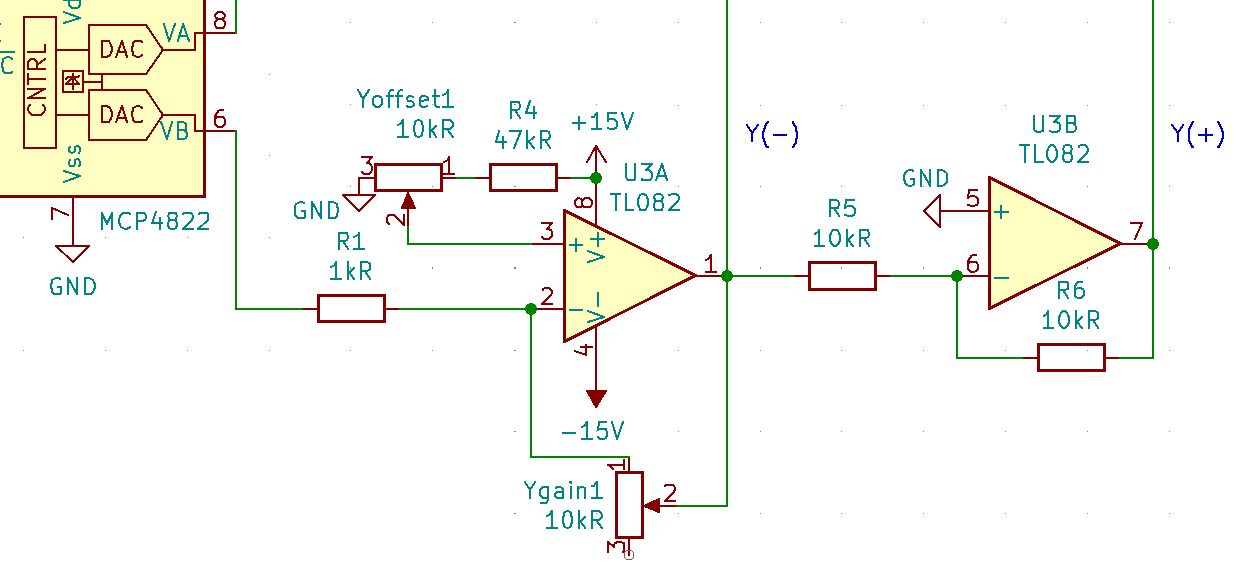
\includegraphics[width=1\textwidth]{img/ilda_amps.png}
  \caption{\label{fig:ilda_amps-scheme} Zapojení čipu TL082 pro jeden kanál řídící desky galvanometrů}
\end{figure}

\subsection{Voltmetr baterií}
Obvod voltmetru baterií je vidět na obrázku \ref{fig:bat_probe}.

\begin{figure}[htb]
  \centering
  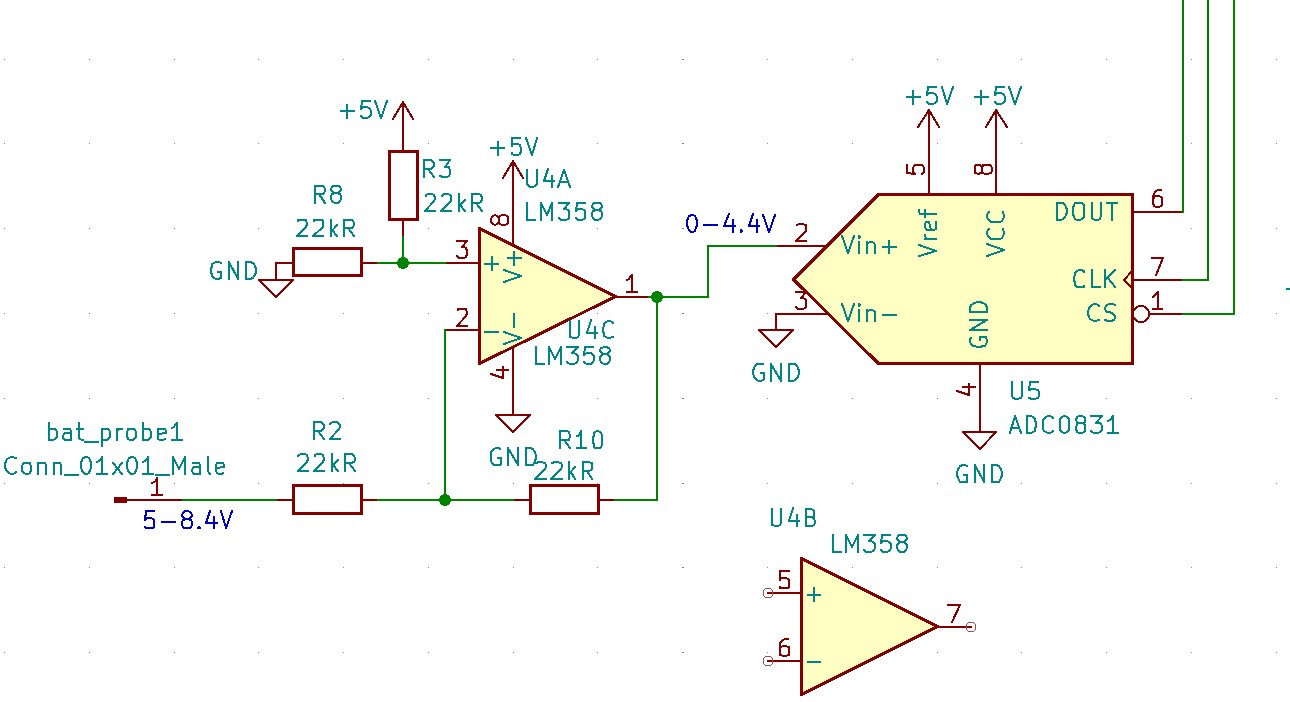
\includegraphics[width=0.6\textwidth]{img/bat_probe.jpg}
  \caption{\label{fig:bat_probe} Schéma obvodu voltmetru baterie}
\end{figure}

Jako voltmetr baterií slouží A/D převodník ADC0831 od firmy Texas Instruments Incorporated~\cite{adc0831-dsh}. Ten je označen U5 a je zapojen společně s operačním zesilovačem LM358 od stejného výrobce, který je označen U4.
Operační zesilovač je zapojen jako rozdílový zesilovač podle zdroje~\cite{odcitacka} tak, aby od napětí baterií, které se může pohybovat v rozsahu 6~V až 8,4~V, odečítal 5~V.
Díky tomu se napětí, která měří A/D převodník pohybují mezi hodnotami 1~V a 3,4~V. S jeho osmibitovým rozlišením a referenčním napětím 5~V v tomto rozpětí může naměřit 122 různých napětí.

A/D převodník tyto data posílá do Raspberry Pi pomocí rozhraní SPI a to s nimi dále pracuje.


\section{Napájení}
Celkové schéma napájení je vidět na obrázku~\ref{fig:power-schem-full}.

\begin{figure}[!h]
  \centering
  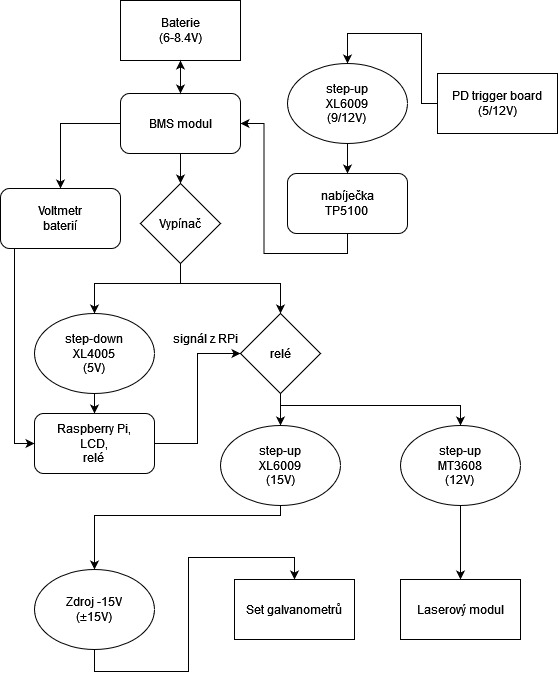
\includegraphics[width=\textwidth]{img/power-schem-full.jpg}
  \caption{\label{fig:power-schem-full} Celkové schéma napájení komponentů projektoru}
\end{figure}

\subsection{Akumulátory}
K napájení projektoru byly využity 4 Lithium-iontové akumulátory Samsung INR 18650 s kapacitou 3450~mAh a jmenovitým napětím 3.7~V. Ty byly zapojeny nejdříve po dvojicích paralelně a následně byly tyto dvojice zapojeny sériově. Konečný článek tedy dosahuje jmenovitého napětí 7,4~V.

\subsection{BMS modul}
Na baterie byl napojen ochranný BMS (Battery management system) modul, který ji chrání před následujícími stavy:
\begin{itemize}
  \item odběr vysokého proudu (zkrat)
  \item přebití
  \item vybití
  \item nevybalancované články
\end{itemize}
Modul články balancuje a v případě, že nastane jiný z nežádoucích stavů, ji odpojí. Modul je na obrázku \ref{fig:BMS}


\begin{figure}[htb]
  \centering
  \begin{minipage}{0.45\textwidth}
    \centering
  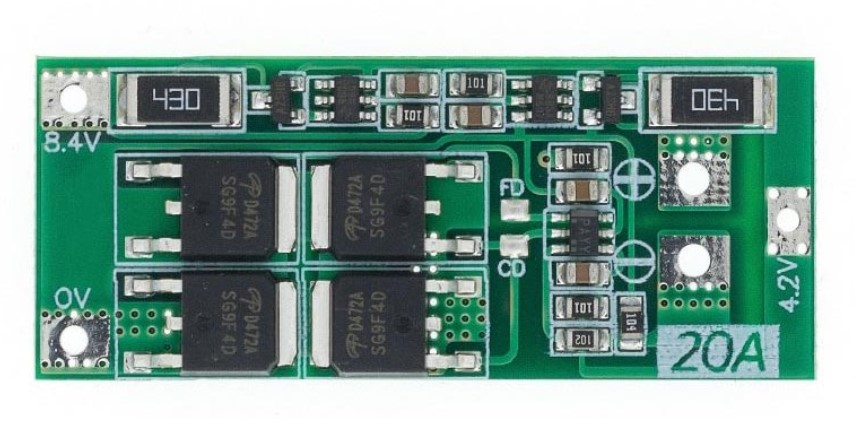
\includegraphics[width=0.8\textwidth]{img/BMS.jpg}
  \caption{\label{fig:BMS} BMS Modul se třemi kontakty pro sérii baterií (0V, 4.2V a 8.4V) a výstupními kontakty ($(+)$ a $(-)$); Převzato z~\cite{laskakit-BMS}}
  \end{minipage}\hfill
  \begin{minipage}{0.45\textwidth}
    \centering
  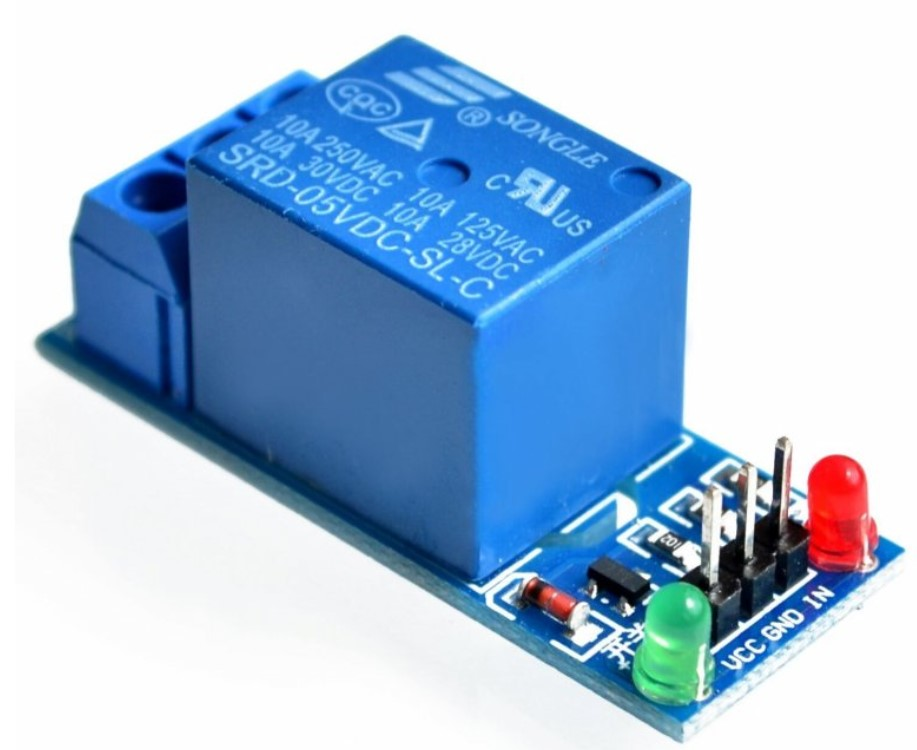
\includegraphics[width=0.8\textwidth]{img/relay.jpg}
  \caption{\label{fig:relay} Relé modul; Převzato z~\cite{laskakit-relay}}
  \end{minipage}
\end{figure}

\subsection{relé modul}
V projektoru byl využit relé modul pro připojování komponentů s vysokým odběrem pouze ve chvílích, kdy jsou využívány. Jedná se o set galvanometrů, laserový modul a větrák, ty jsou připojeny jen ve chvílích, kdy projektor promítá.

Relé modul je ovládán jedním kontaktem spojeným s Raspberry Pi a je umístěn mezi bateriemi a měniči napětí, proto stačí pouze jeden na více napěťových větví. Je vidět na obrazku~\ref{fig:relay}

\subsection{nabíjecí obvod}
Zapojený nabíjecí obvod je vidět na obrázku~\ref{fig:hw_charging_circuit}.

\begin{figure}[htb]
  \centering
  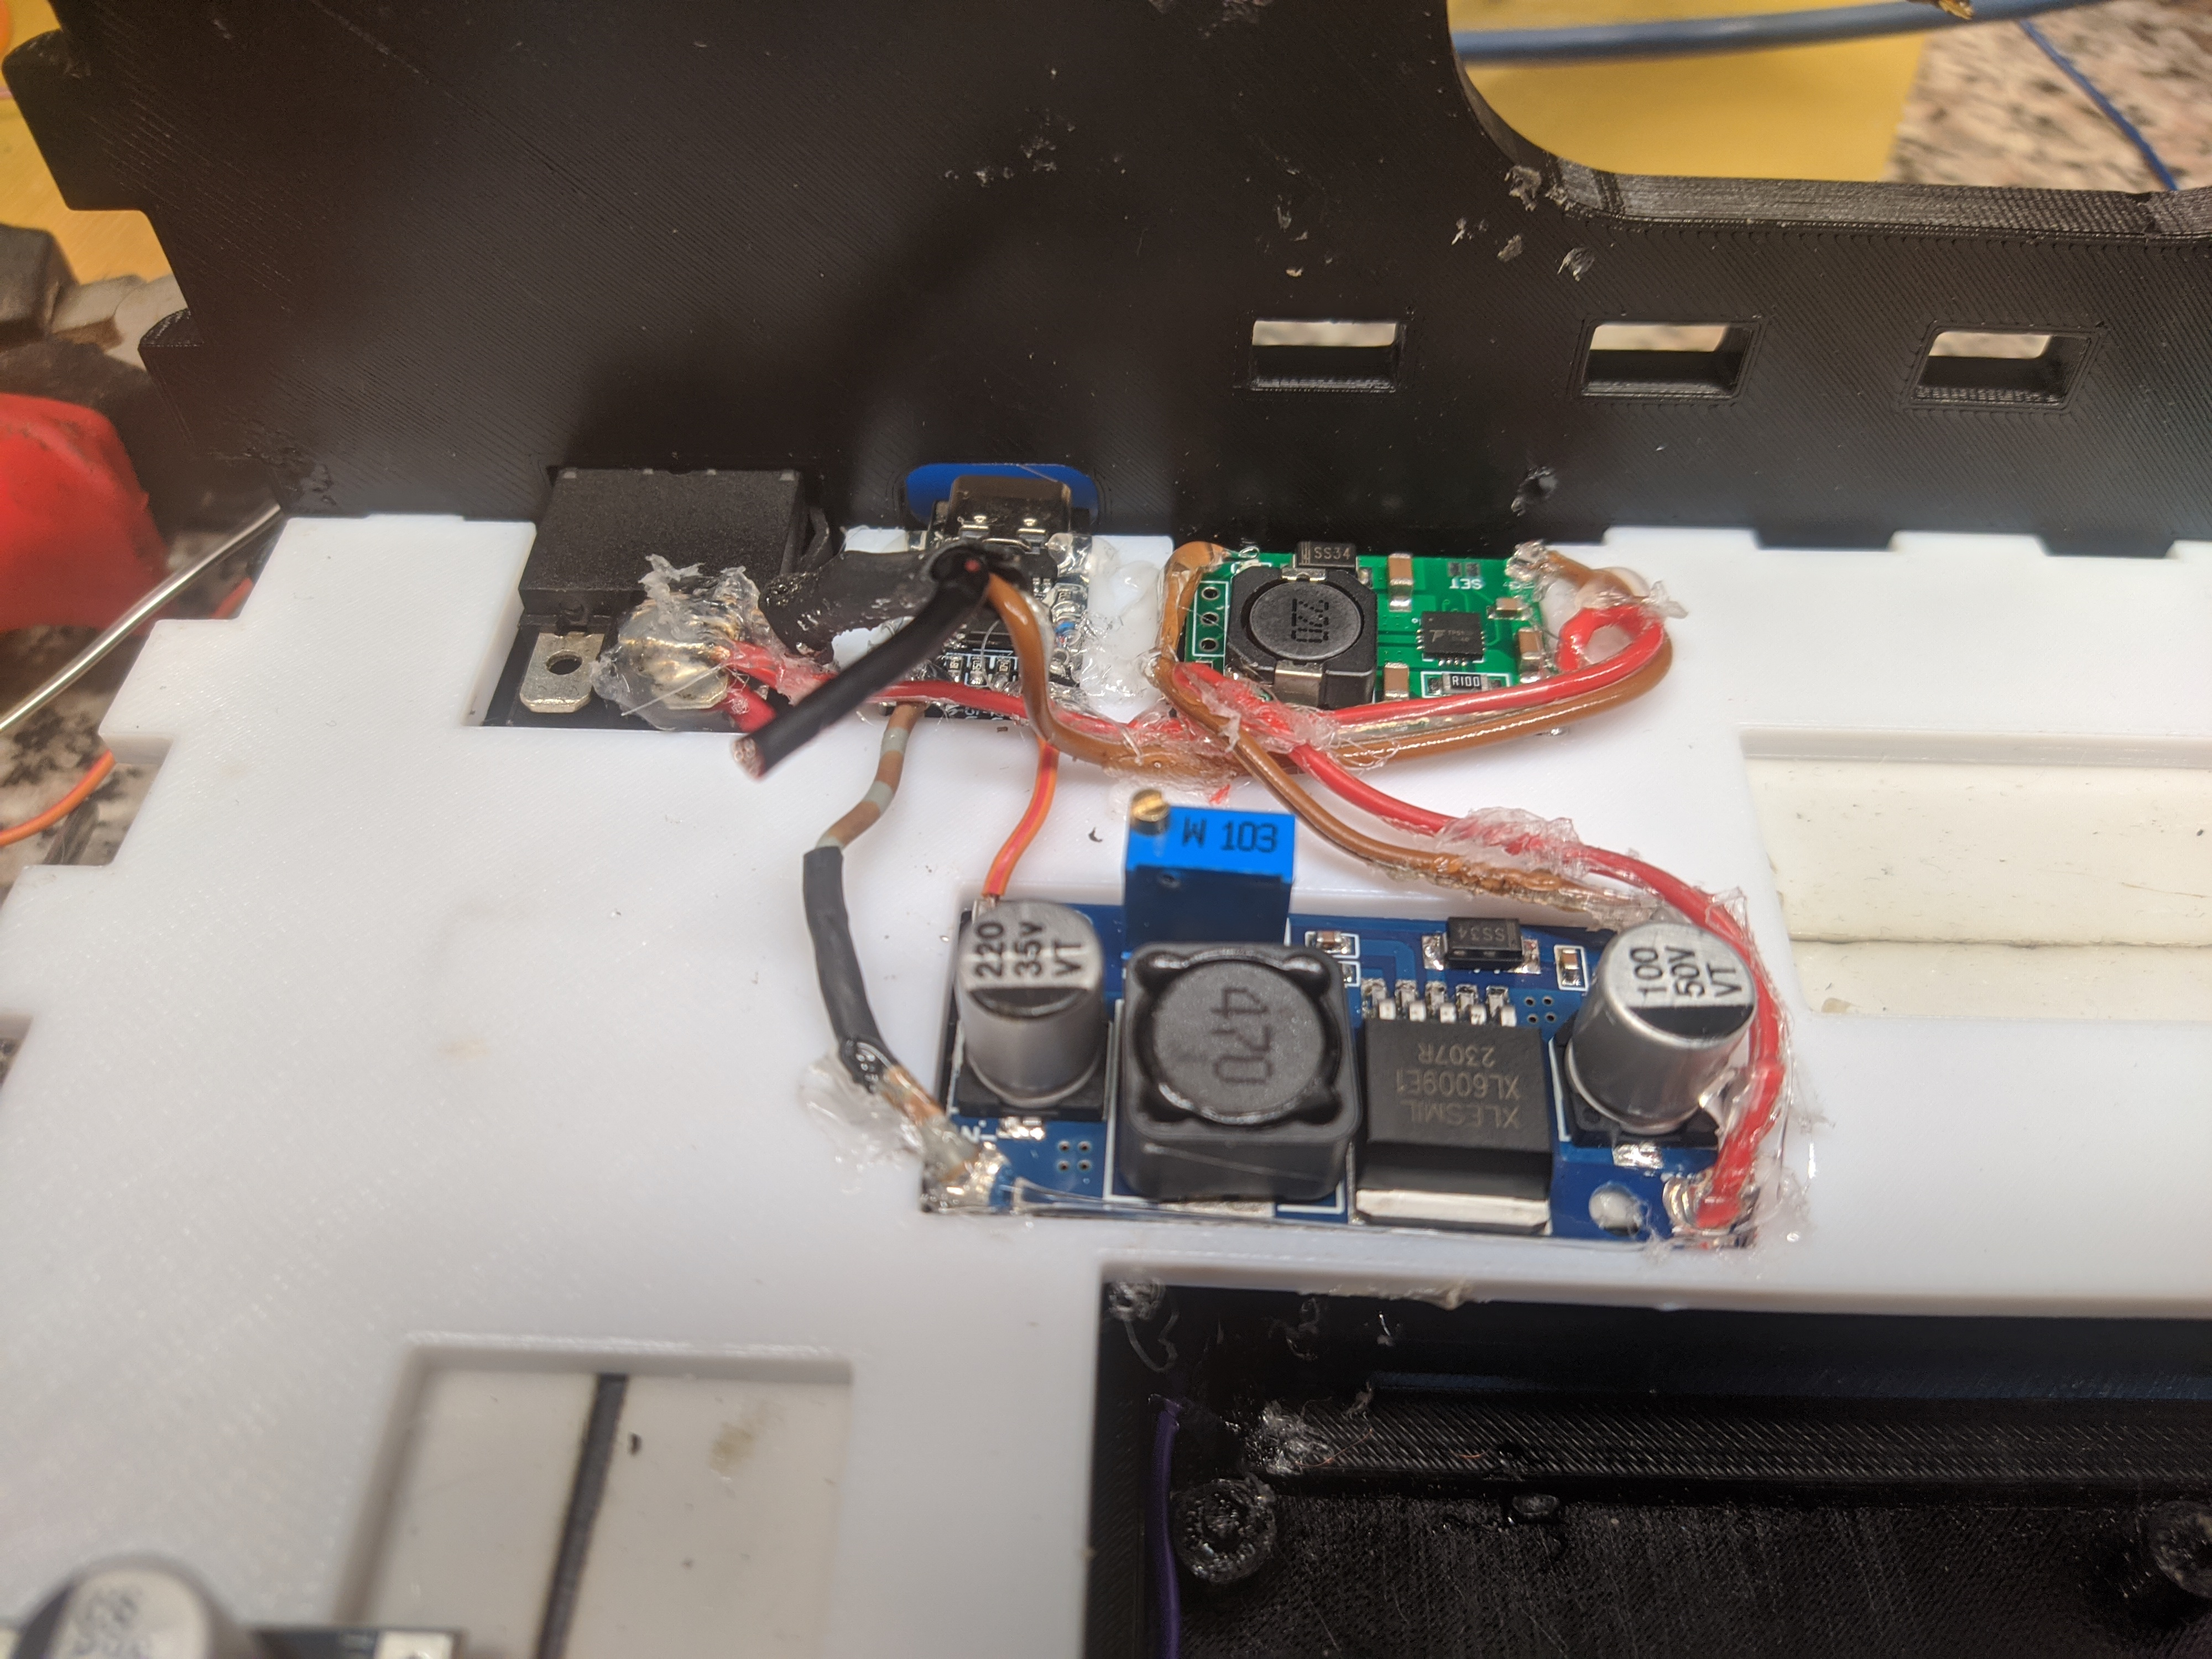
\includegraphics[width=0.8\textwidth]{img/hw_charging_circuit.jpg}
  \caption{\label{fig:hw_charging_circuit} Zapojený nabíjecí obvod}
\end{figure}

\subsubsection{Power Delivery (PD) trigger deska}
K nabíjení baterie je využíván USB-C port podporující moderní protokoly rychlého nabíjení (hlavně Power Delivery a Quick Charge). Ten se nachází na desce s integrovaným obvodem, který přes port komunikuje s adaptérem, pokud adaptér podporuje rychlé nabíjení, čip od něj vyžádá napětí 12~V, které deska převádí na výstupní kontakty viditelné na obrázku~\ref{fig:PDtrig}. Protože deska \uv{vyvolá} dané napětí, označuje se PD trigger board (deska).

\begin{figure}[htb]
  \centering
  \begin{minipage}{0.3\textwidth}
    \centering
  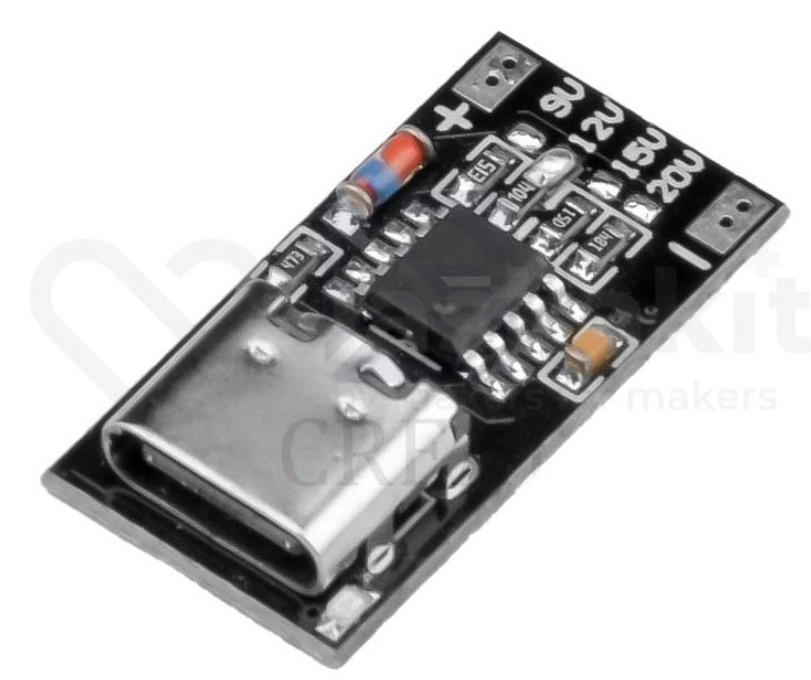
\includegraphics[width=1\textwidth]{img/PDtrig.jpg}
  \caption{\label{fig:PDtrig} Power Delivery trigger board; Převzato z~\cite{laskakit-PD}}
  \end{minipage}\hfill
  \begin{minipage}{0.3\textwidth}
    \centering
  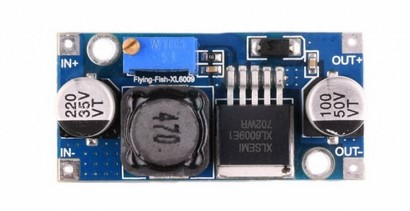
\includegraphics[width=1\textwidth]{img/XL6009.jpg}
  \caption{\label{fig:XL6009} step-up měnič s čipem XL6009; Převzato z~\cite{laskakit-XL6009}}
  \end{minipage}
  \begin{minipage}{0.3\textwidth}
    \centering
    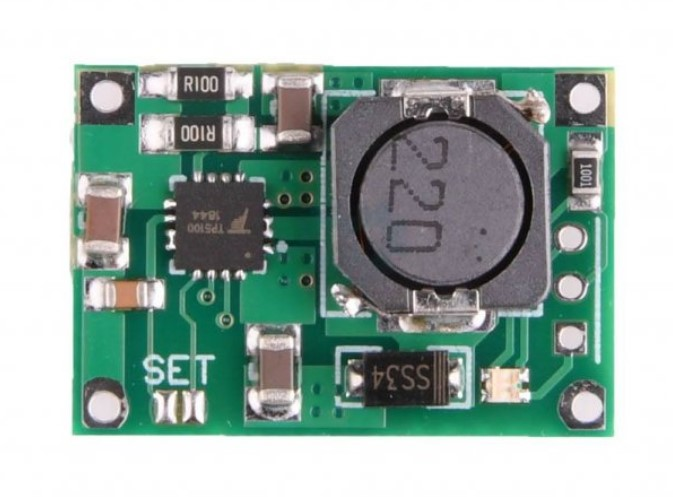
\includegraphics[width=0.8\textwidth]{img/TP5100.jpg}
    \caption{\label{fig:TP5100} Modul nabíječky dvou sériově zapojených Li-ion baterií; Převzato z~\cite{laskakit-TP5100}}
  \end{minipage}
\end{figure}

\subsubsection{Step up měnič s čipem XL6009}
Pokud ovšem připojený adaptér nepodporuje žádný rychlonabíjecí protokol, na výstupech desky bude napětí pouze 5~V Na kterém standartně běží USB připojení. Proto je k PD trigger board připojen step-up měnič nastavený na 9~V.
Pokud z PD desky bude vycházet napětí 5V, step-up jej zvýší na 9V. Pokud z PD desky bude vycházet 12V, napětí step-up projde beze změny.

\subsubsection{tp5100}
K ovládání průběhu nabíjení byl využit modul pro nabíjení Li-ionových baterií s čipem TP5100. Ten zajišťuje konstantní proud a napětí, které posílá na kontakty BMS obvodu. Další z jeho funkcí je automatické ukončení nabíjení ve chvíli, kdy baterie dosáhnou napětí 8.4~V. Je to jedinečný modul, který umožňuje nabíjení dvoučlánkových lithium-iontových akumulátorů.

\subsection{Vypínač}
K bateriím je neustále připojený jen BMS modul a nabíjecí obvod, všechny ostatní obvody jsou přemostěny vypínačem. Je tedy možné baterie nabíjet i když jsou všechny ostatní obvody odpojené. Vypínač je vidět na obrázku~\ref{fig:hw_charging_circuit}.

\subsection{Napěťové větve}
Různé komponenty projektoru pracují s různými napětími. Je tedy potřeba napětí baterií převést na několik napěťových větví. Jedná se o větve:

\begin{itemize}
  \item 5V --- Napětí Raspberry Pi, LCD a relé modulu; Zajištěno step-down měničem s čipem XL4005 (Viz obrázek~\ref{fig:XL4005}.)
  \item 12V --- Napětí Laserového modulu; Zajištěno step-up měničem s čipem MT3608 (Viz obrázek~\ref{fig:MT3608}.)
  \item symetrické napětí $\pm{}15$~V --- Napětí řídící desky galvanmetrů; Kladná větev zajištěna step-up měničem s čipem XL6009 (Viz obrázek~\ref{fig:XL6009}.), záporná větev zajištěna obvodem zdroje -15~V na HAT DPS (Viz kapitola~\ref{sec:negative-ps})
\end{itemize}


\begin{figure}[htb]
  \centering
  \begin{minipage}{0.45\textwidth}
    \centering
  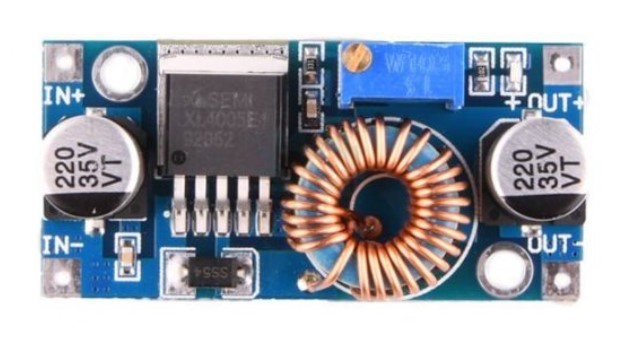
\includegraphics[width=0.8\textwidth]{img/XL4005.jpg}
  \caption{\label{fig:XL4005} step-down měnič s čipem XL4005; Převzato z~\cite{laskakit-XL4005}}
  \end{minipage}\hfill
  \begin{minipage}{0.45\textwidth}
    \centering
  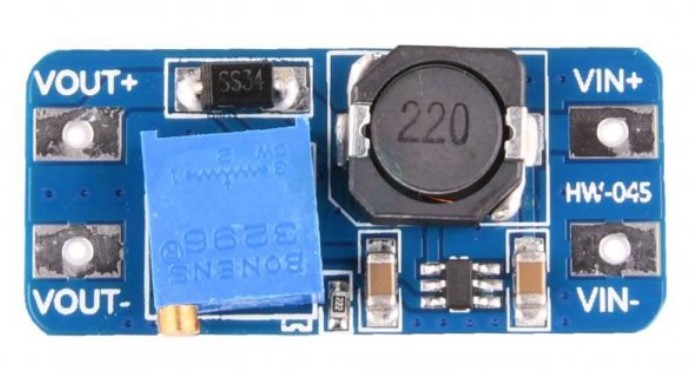
\includegraphics[width=0.8\textwidth]{img/MT3608.jpg}
  \caption{\label{fig:MT3608} step-up měnič s čipem MT3608; Převzato z~\cite{laskakit-MT3608}}
  \end{minipage}
\end{figure}


\section{Pouzdro}

V~rámci popularizace technologie se~může hodit projektor předvádět na~různých místech. Proto bude potřeba, aby~byl projektor přenosný a~při přemisťování se~nerozbil.

Pouzdro je~tedy navrženo tak, aby~bylo odolné proti nárazům a~zachovalo všechny součásti v~bezpečí. Každá součástka má své místo, kde~je~držena ze~všech stran. Pro~výrobu pouzdra by~bylo vhodné využít technologii 3D tisku. Ta~umožňuje tvorbu komplexních geometrických tvarů přímo pro~potřeby konkrétního modelu a~zároveň umožňuje snadnou iteraci a~úpravu designu pouzdra při nalezení chyb.

Pouzdro bylo navrženo v~programu Autodesk Fusion.

\subsection{Priority designu} \label{sec:krabick-design-priorities}
\subsubsection{Chlazení}
Největší část projektoru je~hliníkový chladič s~větrákem. Už od~začátku práce byl~tento chladič vybrán, aby~byl připevněn k~řídící desce galvanometrů. Problematika jejího zahřívání je~popsaná v~kapitole~\ref{sec:galvoboard-chips-heating-up}.
Jak bylo popsáno v~této kapitole, na~řídící desce galvanometrů je~připevněna hliníková destička, která chladí čipy. Chladič byl~připevněn právě na~ni.

Aktivní chladič\footnote{Chladič s~větrákem, který aktivně vytváří proud vzduchu.} se~ale~hodí i~pro~ostatní součástky. Vzduch, který nasaje, je~totiž distribuován celou vnitřní konstrukcí projektoru a~chladí tak~všechny vnitřní součástky. Tomuto proudění byla věnována zvláštní pozornost při designu konstrukce pouzdra.

\subsubsection{Přístup k~portům Raspberry Pi}
Aby bylo možné je~používat, je~potřeba zajistit jednoduchý přístup k~portům Raspberry Pi. Dále je~potřeba od~nich odlišit nabíjecí port.

\subsubsection{Modularita, jednoduchá konstrukce}
Pouzdro bylo designováno, také aby~bylo modulární. Aby~bylo možné při prototypování vyměnit pouze jednu součástku, která nesedí, místo tisknutí celého pouzdra od~začátku. S~modularitou bylo zároveň dosaženo jednoduché konstrukce, v~jakékoliv části stavby je~možné dočasně odstranit díly, aby~bylo možné upravit připevnění vnitřní elektroniky.

\subsection{Konstrukce}
Pouzdro se~skládá ze~čtyř vertikálních stěn s~otvory, do~kterých zapadají horizontální desky. Horizontální desky v~sobě mají vždy z~vrchní strany vyhloubené prohlubně, do~kterých pasují elektronické součástky, které na~nich leží. Díky tomu se~elektronické součástky při pohybu projektoru volně nepohybují ve~vnitřních prostorách.

\begin{figure}[htb]
  \centering
  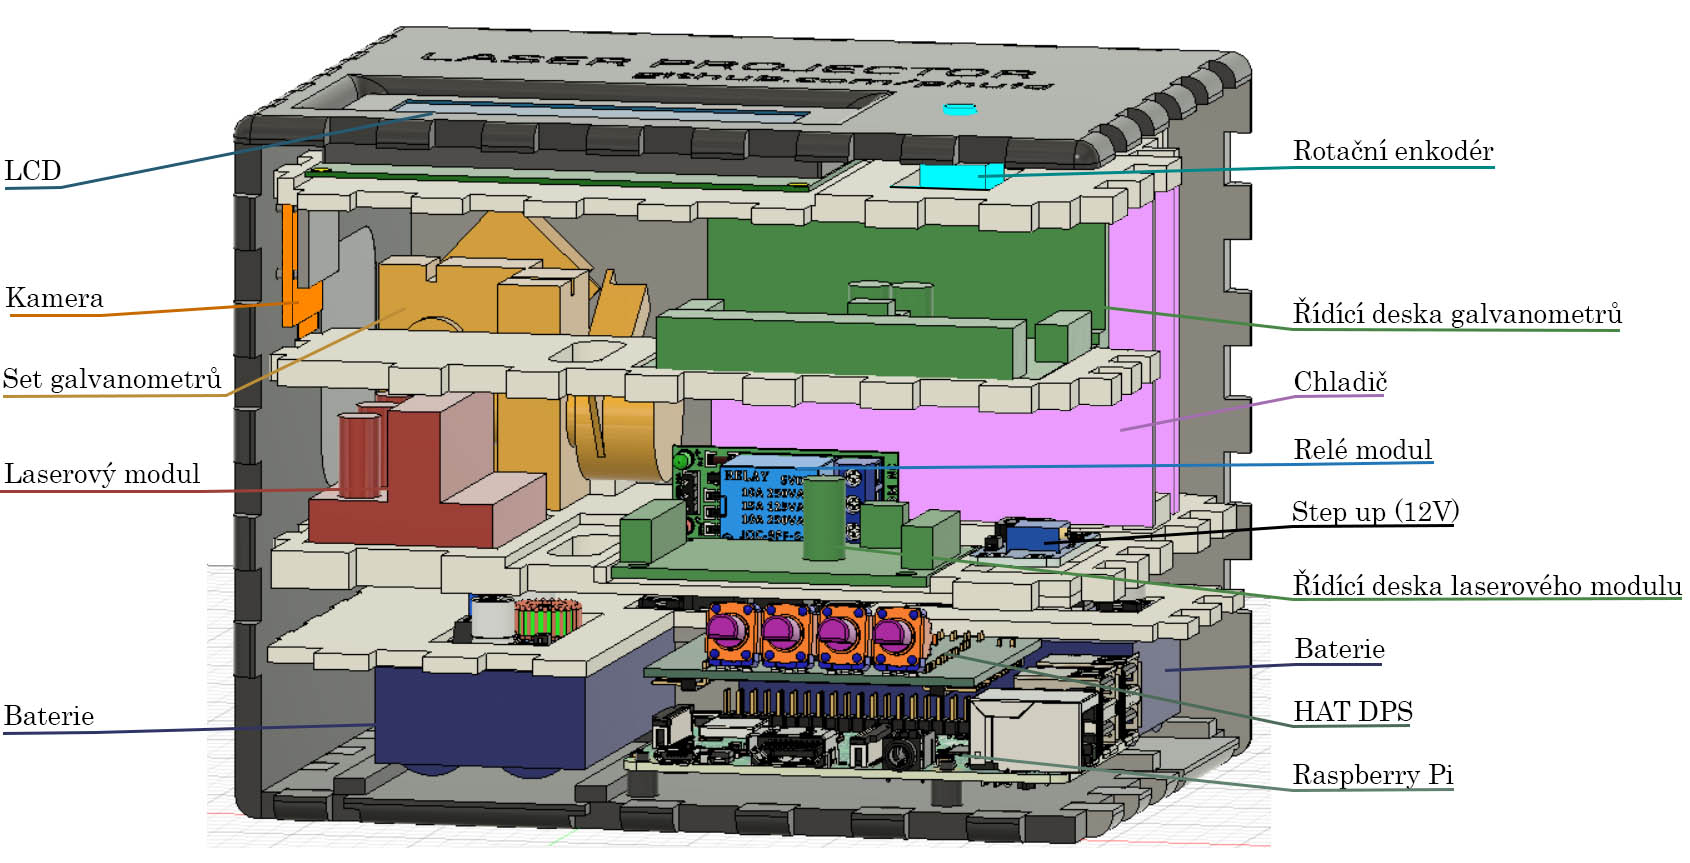
\includegraphics[width=1\textwidth]{img/case-sideview.jpg}
  \caption{\label{fig:case-sideview} Pohled do~projektoru s~odstraněnou přední stěnou v~programu Autodesk Fusion}
\end{figure}

Tyto prohlubně jsou hlavní důvod, proč byl~k~výrobě dílů využit 3D tisk místo například laserového řezání.

Elektronika je~v~prohlubních často držena i~lepidlem z~tavné pistole.
To bylo přidáno s~původním cílem upevnit k~elektronice kabely z~ní vedoucí i~za~izolaci. Kdyby kabely držely jen~za~vodičové drátky k~elektronice připájené, drátky by~se~v~průběhu času kvůli vibracím při přenášení polámaly.

Jak je~vidět na~obrázku~\ref{fig:case-sideview}, pouzdro je~rozděleno do~pěti pater. Jednotlivá patra nezabírají celou horizontální plochu projektoru. Často spojují pouze tři ze~čtyř stěn, nebo jsou v~nich otvory, kterými může proudit vzduch. V~prvním patře se~nachází baterie (zvýrazněny modře), destička s~BMS obvodem a~v~neposlední řadě Raspberry Pi.
Na~něm je~připevněná HAT~deska plošných spojů, která zasahuje do~druhého patra. Druhé patro je~vidět na~obrázku~\ref{fig:hw_layer0} a~nachází se~v~něm obvod nabíjení baterie (PD trigger deska, step up~měnič a~nabíječka Li-ion článků).
Dále se~v~něm nachází step down měnič napájející Raspberry Pi~a~step up~měnič napájející galvanometry.
\fxnote{tecka @ obr.\ref{fig:hw_layer0}} 
\begin{figure}[htb]
  \centering
  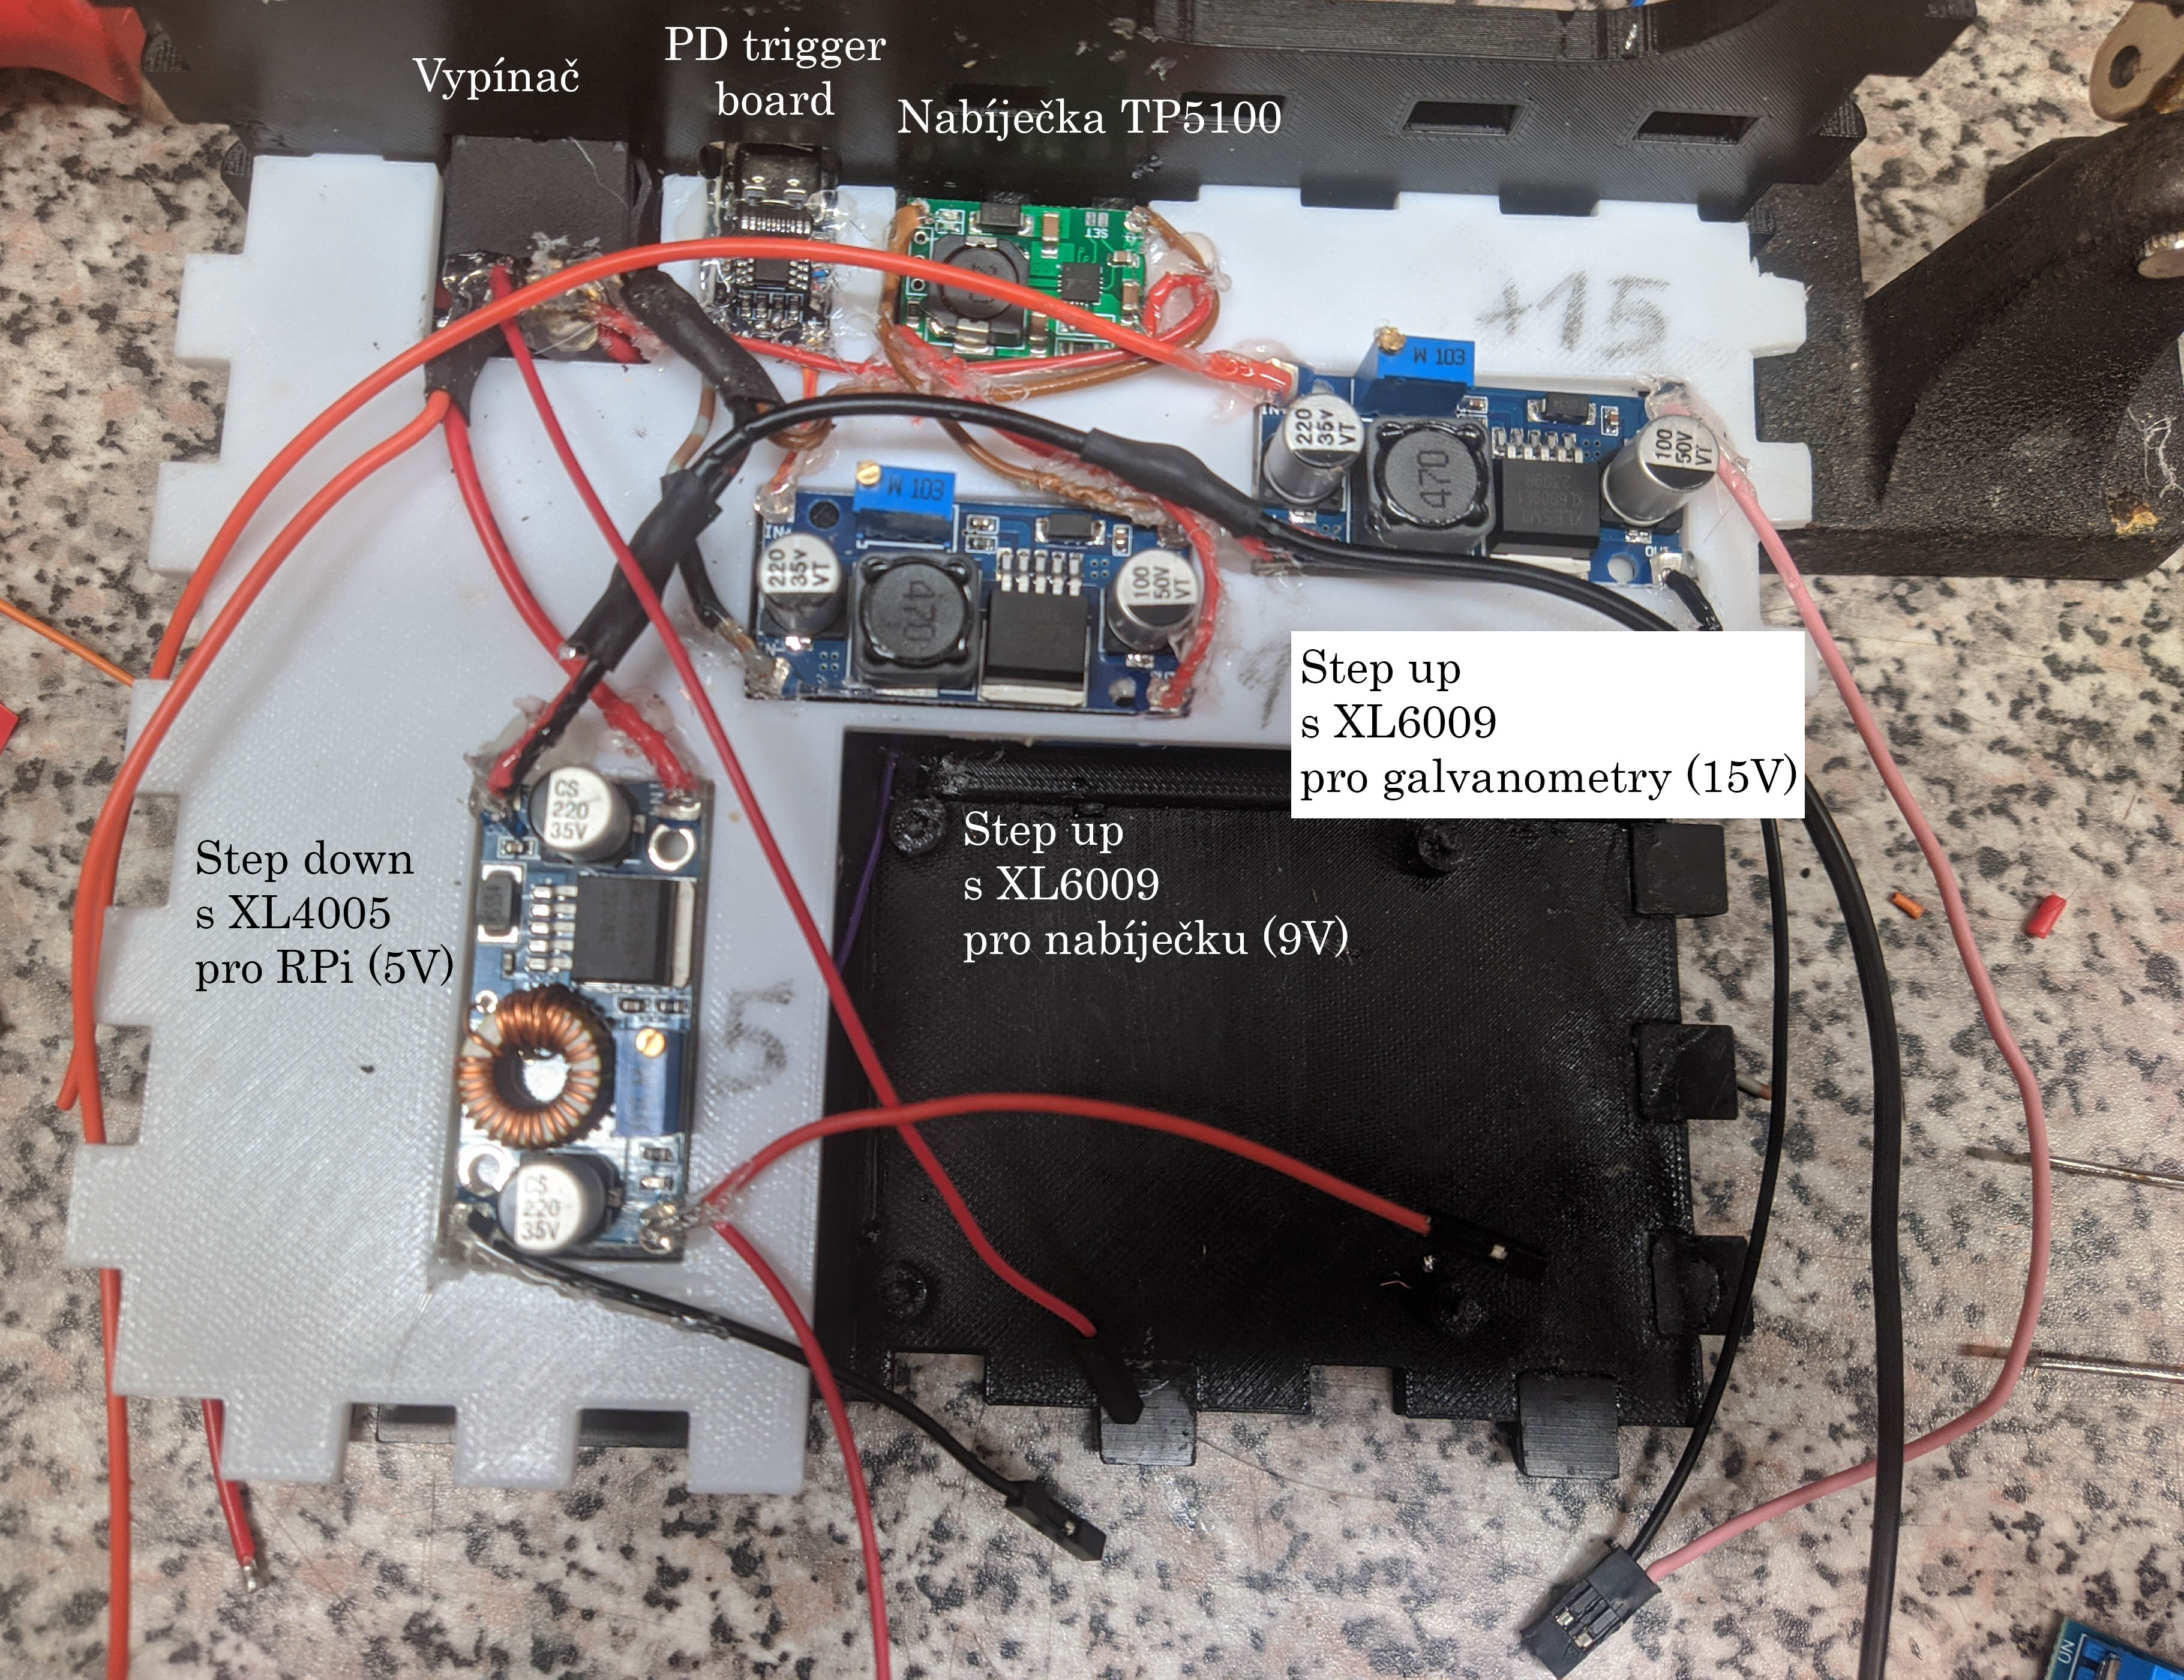
\includegraphics[width=0.8\textwidth]{img/hw_layer0.jpg}
  \caption{\label{fig:hw_layer0} Kompletně nainstalované druhé patro (Na obrázku je~modul TP5100 zapojen s~opačnou polaritou, ve~výrobku byla chyba opravena, ale~tato fotka je~stále nejlepší ilustrace.)}
\end{figure}

Ve třetím patře je~upeněn chladič, foukající na~nabíjecí obvod a~step up~měniče pod~ním, set~galvanometrů (zvýrazněn žlutě), laserový modul (zvýrazněn červeně) a~jeho řídící deska (zvýrazněna zeleně), step up~měnič pro~laser a~relé modul.  
Galvanometry zasahují až do~čtvrtého patra, kde~je~upevněna jejich řídící deska. Ta~je~mimo jiné připevněna na~chladič párem šroubků viditelných na~obrázku~\ref{fig:hw_galvoboard} ze~strany \pageref{fig:hw_galvoboard}, mezi desku a~chladič byla aplikována teplovodivá pasta. V~prostorách čtvrtého patra je~také na~stěnu upevněna kamera.
V pátém patře se~nachází LCD~a~rotační enkodér.

V horizontálních deskách oddělujících patra od~sebe jsou otvory pro~vzduch, jak~je~zmíněno v~sekci~\ref{sec:krabick-design-priorities}, také na~přední stěně pouzdra jsou otvory pro~vyfukování vzduchu. Na~přední stěně je~také otvor pro~přístup k~potenciometrům na~HAT~DPS a~otvor pro~přístup k~portům Raspberry Pi, ten~je~i~na~pravé boční stěně.
Na~zadní stěně je~otvor pro~nasávání vzduchu větrákem, vypínač a~otvory pro~USB-C port PD~trigger desky a~statusové diody nabíječky TP5100. Na~levé boční stěně jsou pak~otvory pro~kameru a~laserový výstup galvanometrů. Ve~dně jsou otvory pro~výmněnu baterií a~ve~stropní stěně jsou otvory pro~LCD a~rotační enkodér.

\begin{figure}[htb]
  \centering
  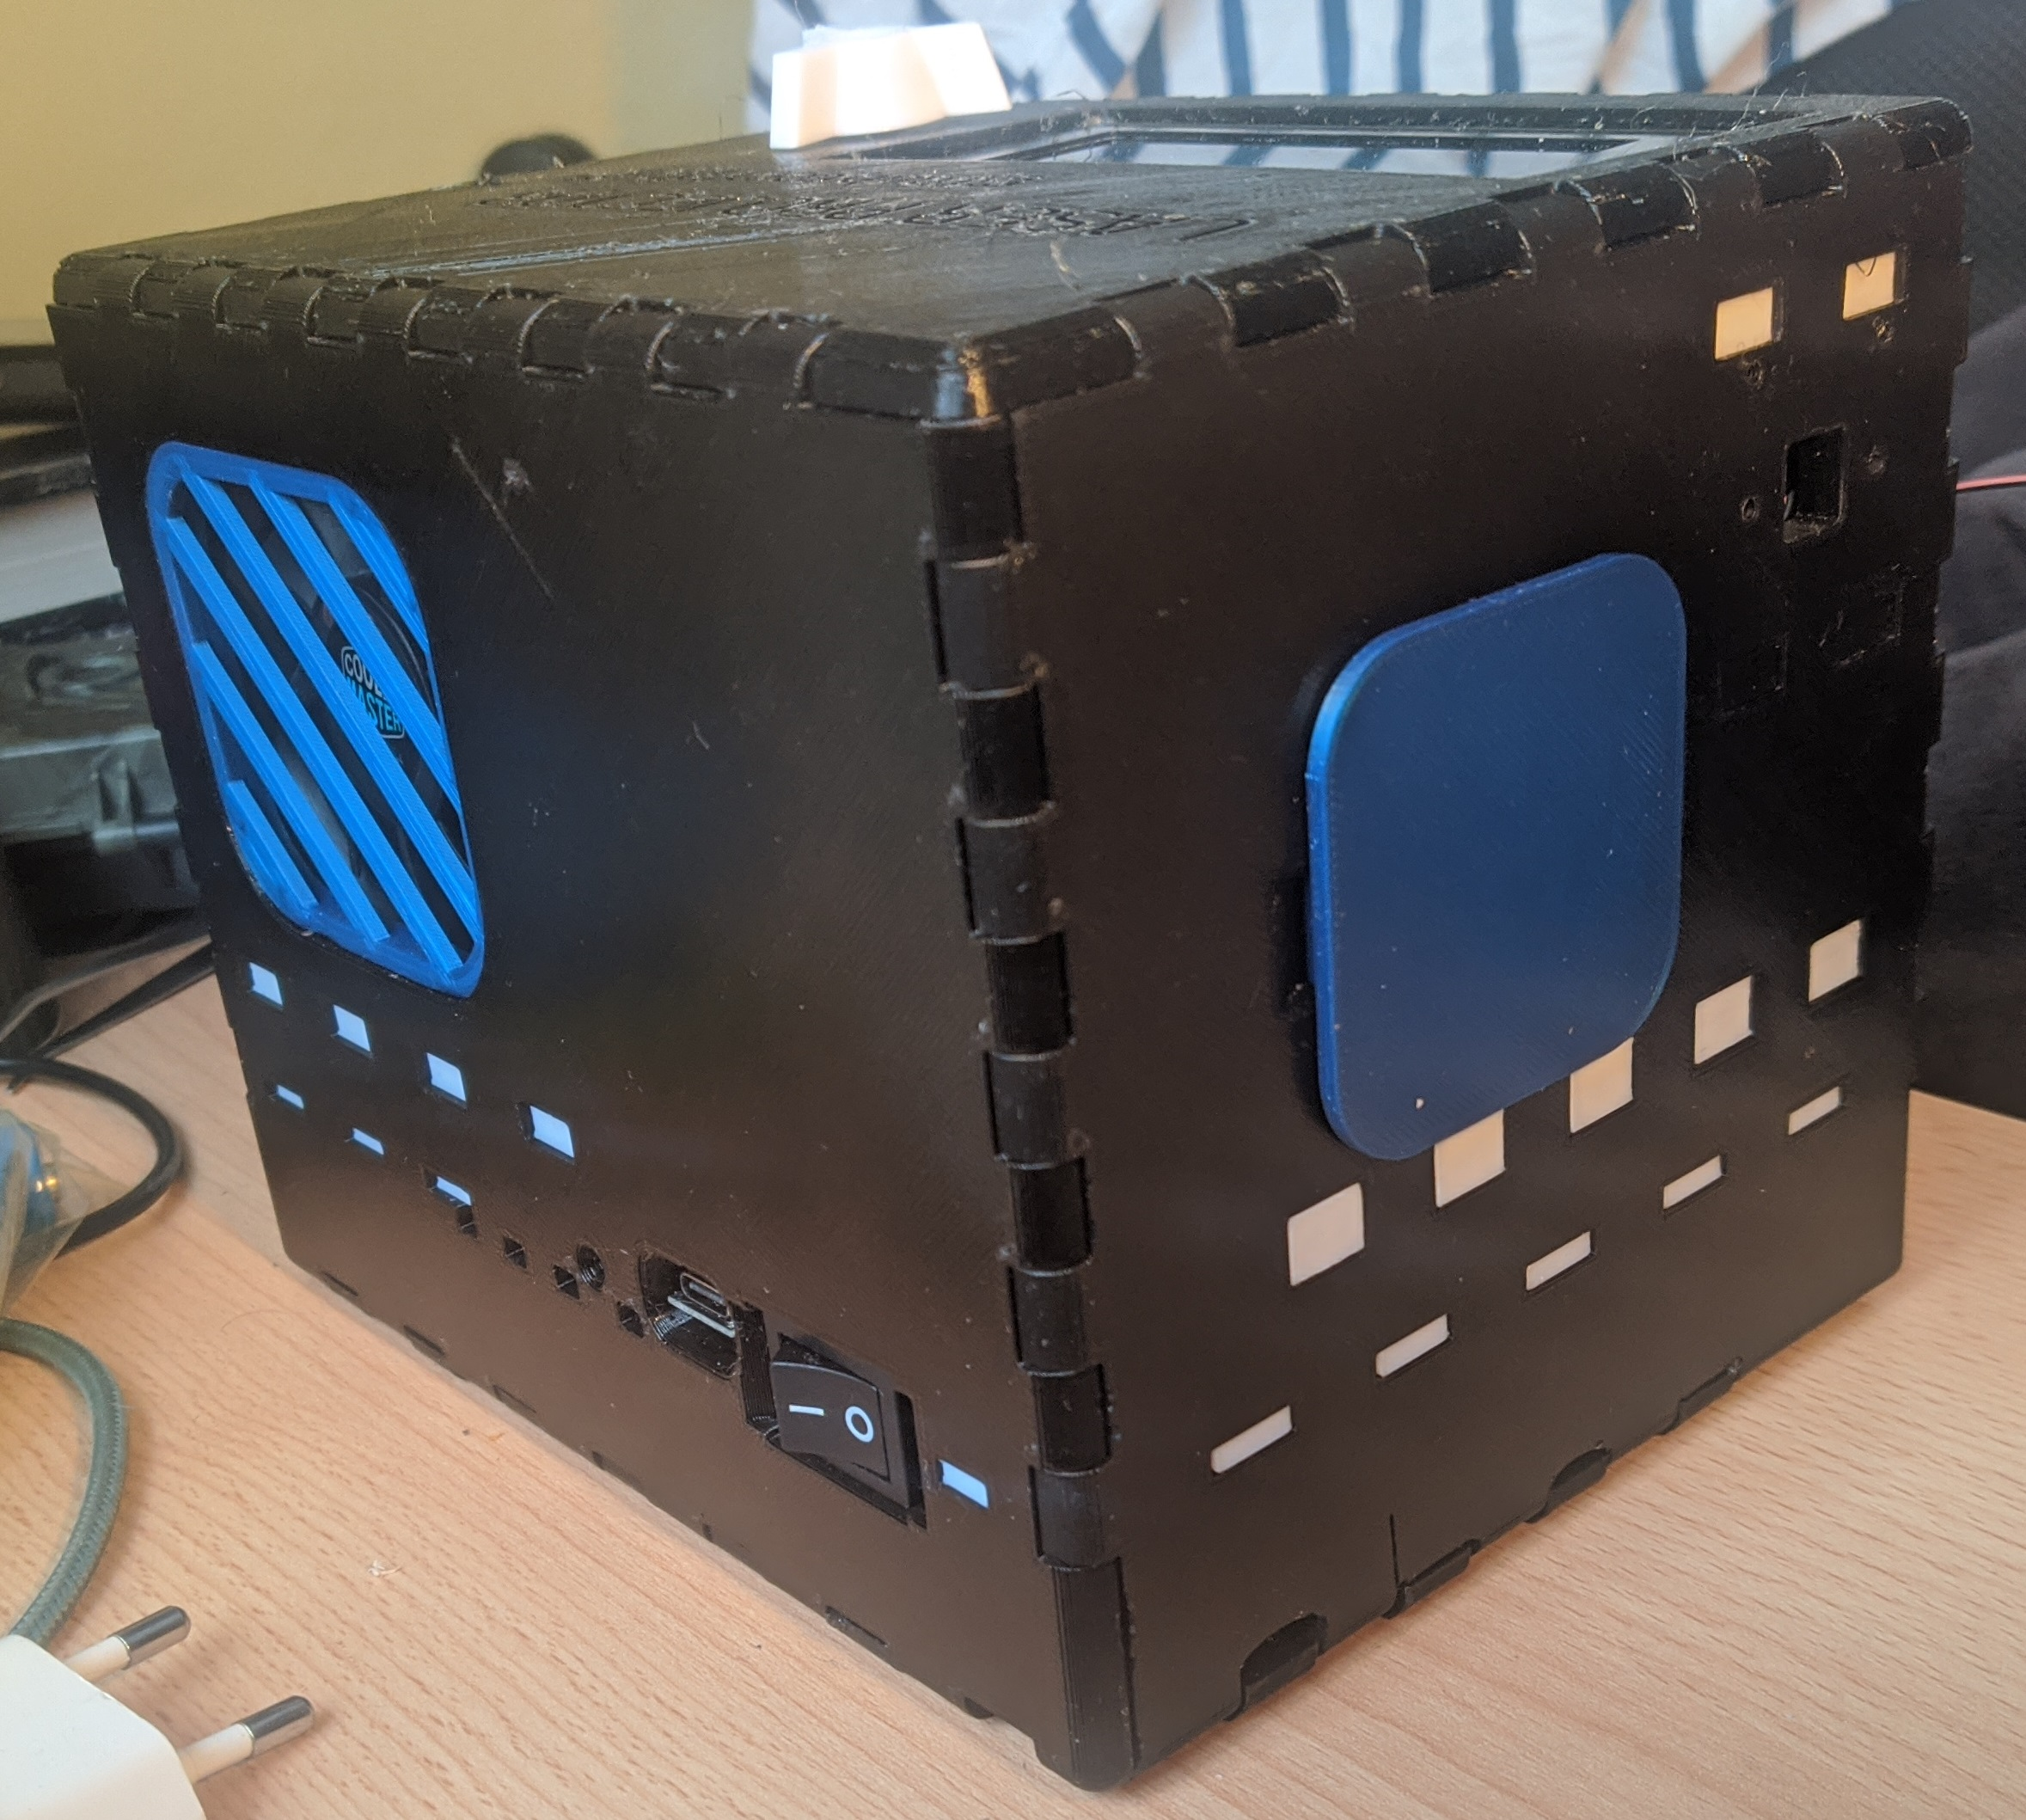
\includegraphics[width=0.8\textwidth]{img/hw_sides_backleft.jpg}
  \caption{\label{fig:hw_sides_backleft.jpg} Pohled na~projektor ze~strany hrany sousedící se~zadní a~pravou boční stěnou}
\end{figure}

\fxnote{fotka zepredu a~zprava}



\fxnote{TODO cos udelal svyho vlastne a~jak to~facha}

\section{cooler}

\section{napájení}
\fxnote{TODO ay~tak co, zvladls to~dat na~baterky?}
